% Created 2017-09-20 Wed 13:20
% Intended LaTeX compiler: pdflatex
\documentclass[presentation]{beamer}
\usepackage{listings}
\usepackage{verbatim}
\usepackage{algorithm2e}
\usepackage{amsmath}
\usepackage{tikz}
\usepackage{hyperref}
\usetheme[height=20pt]{Rochester}
\date{\today}
\title{Search}
\author{A.I. Society at UTDallas}
\begin{document}
\begin{frame}
  \maketitle
\end{frame}
\begin{frame}{Outline}
  \tableofcontents
\end{frame}
\section{Setup}
\begin{frame}
  \frametitle{Setup}
    
\end{frame}
\section{Introduction}
\begin{frame}
  \frametitle{Introduction}
  What does it mean to search?\\
  \begin{figure}
    \centering
    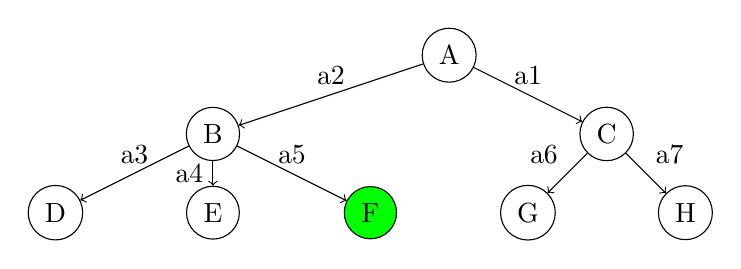
\begin{tikzpicture}
      \node[shape=circle,draw=black](A) at (0,0) {A};
      \node[shape=circle,draw=black](B) at (-3, -1) {B};
      \node[shape=circle,draw=black](C) at (2, -1) {C};
      \node[shape=circle,draw=black](D) at (-5,-2) {D};
      \node[shape=circle,draw=black](E) at (-3, -2) {E};
      \node[shape=circle,draw=black,fill=green](F) at (-1, -2) {F};
      \node[shape=circle,draw=black](G) at (1,-2) {G};
      \node[shape=circle,draw=black](H) at (3, -2) {H};

      \path [->] (A) edge node[above] {a1} (C);
      \path [->] (A) edge node[above] {a2} (B);
      \path [->] (B) edge node[above] {a3} (D);
      \path [->] (B) edge node[left] {a4} (E);
      \path [->] (B) edge node[above] {a5} (F);
      \path [->] (C) edge node[above left] {a6} (G);
      \path [->] (C) edge node[above right] {a7} (H);
    \end{tikzpicture}
  \end{figure}
\end{frame}

\begin{frame}{Problems}
  \begin{itemize}
  \item What Problems can be solved by searching?
    \begin{itemize}
    \item <1-> Chess
      \begin{itemize}
      \item <7-> Branching Factor: $\approx 35$
      \end{itemize}
    \item <2-> Mazes
      \begin{itemize}
      \item <8-> Branching Factor: $3$
      \end{itemize}
    \item <3-> Computer Algebra
      System
      \begin{itemize}
      \item <9-> Branching Factor:
        idk lol
      \end{itemize}
    \end{itemize}
  \item What Problems should we NOT use search?
    \begin{itemize}
    \item <4-> Travelling salesman problem
      \begin{itemize}
      \item <10-> Branching Factor: $O(N)$
      \end{itemize}
    \item <5-> Go
      \begin{itemize}
      \item <11-> Branching Factor: $\approx 250$
      \end{itemize}
    \item <6-> Program Synthesis
      \begin{itemize}
      \item <12-> Very costly goal test!
      \end{itemize}
    \end{itemize}
  \end{itemize}
\end{frame}

\section{Breadth First and Depth First Search}
\begin{frame}{Breadth First}
  \begin{figure}
    \centering
    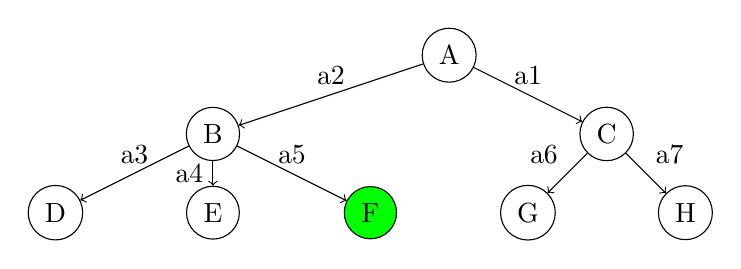
\begin{tikzpicture}[]
      \node[shape=circle,draw=black](A) at (0,0) {A};
      \node[shape=circle,draw=black](B) at (-3, -1) {B};
      \node[shape=circle,draw=black](C) at (2, -1) {C};
      \node[shape=circle,draw=black](D) at (-5,-2) {D};
      \node[shape=circle,draw=black](E) at (-3, -2) {E};
      \node[shape=circle,draw=black,fill=green](F) at (-1, -2) {F};
      \node[shape=circle,draw=black](G) at (1,-2) {G};
      \node[shape=circle,draw=black](H) at (3, -2) {H};

      \path [->] (A) edge node[above] {a1} (C);
      \path [->] (A) edge node[above] {a2} (B);
      \path [->] (B) edge node[above] {a3} (D);
      \path [->] (B) edge node[left] {a4} (E);
      \path [->] (B) edge node[above] {a5} (F);
      \path [->] (C) edge node[above left] {a6} (G);
      \path [->] (C) edge node[above right] {a7} (H);
    \end{tikzpicture}
  \end{figure}
  \begin{tabular}{c | l | l}
    Current Node & Queue & New Queue \\ \hline
    A & [] & [B C] \\
    B & [C] & [C D E F] \\
    C & [D E F] & [D E F] \\
    D & [E F] & [E F] \\
    E & [F] & [F] \\
    F & [] & Done! \\
  \end{tabular}
\end{frame}

\begin{frame}
  \frametitle{Breadth First}
  \begin{itemize}
  
  \item Utilizes a Queue: First in, First Out
  \end{itemize}
  % \scriptsize \verbatiminput{../src/bfs.py}
  \normalsize
  \begin{itemize}
  \item What's missing?
    \begin{itemize}
    \item<2-> goal\_test() 
    \item<2-> successors() 
    \end{itemize}
  \end{itemize}

  
\end{frame}

\begin{frame}
  \frametitle{Depth First}
  \begin{figure}
    \centering
    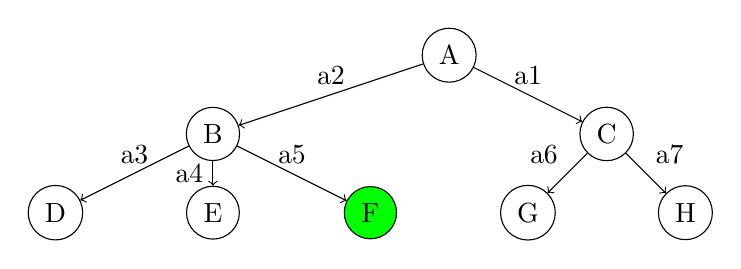
\begin{tikzpicture}[]
      \node[shape=circle,draw=black](A) at (0,0) {A};
      \node[shape=circle,draw=black](B) at (-3, -1) {B};
      \node[shape=circle,draw=black](C) at (2, -1) {C};
      \node[shape=circle,draw=black](D) at (-5,-2) {D};
      \node[shape=circle,draw=black](E) at (-3, -2) {E};
      \node[shape=circle,draw=black,fill=green](F) at (-1, -2) {F};
      \node[shape=circle,draw=black](G) at (1,-2) {G};
      \node[shape=circle,draw=black](H) at (3, -2) {H};

      \path [->] (A) edge node[above] {a1} (C);
      \path [->] (A) edge node[above] {a2} (B);
      \path [->] (B) edge node[above] {a3} (D);
      \path [->] (B) edge node[left] {a4} (E);
      \path [->] (B) edge node[above] {a5} (F);
      \path [->] (C) edge node[above left] {a6} (G);
      \path [->] (C) edge node[above right] {a7} (H);
    \end{tikzpicture}
  \end{figure}
  \begin{tabular}{ c | l | l}
    Current Node & Stack & New Stack \\ \hline
    A & [] & [B, C] \\
    C & [B] & [B, G, H] \\
    H & [B, G] & [B, G] \\
    G & [B] & [B] \\
    B & [] & [D E F] \\
    F & [D E] & Done! \\
  \end{tabular}
\end{frame}
\begin{frame}{Example Time!}
  TODO: live coding of maze solver
\end{frame}
\begin{frame}
  \frametitle{What's the
    Difference?}
  \begin{itemize}
    
  \item Average branching factor:
    $b$
  \item Depth of goal node: $d$
  \item<1-> BFS
    \begin{itemize}
    \item<2-> Runtime: $O(d^b)$
    \item<3-> Space: $O(d^b)$
    \end{itemize}
    
  \item<4-> DFS
    \begin{itemize}
    \item<5-> Runtime: $O(d^b)$
    \item<6-> Space: $O(d)$
    \end{itemize}
  \end{itemize}
\end{frame}
\section{Bidirectional Search}
\begin{frame}{Bidirectional Search}
  \begin{itemize}
  \item reduce nodes evaluated
  \item $\frac{2a}{A} =
    \frac{2\pi(r)^2}{\pi(2r)^2} =
    \frac{2\pi r^2}{4\pi r^2} = \frac{1}{2}$
  \item only works (well) with
    unique goal state
  \end{itemize}
  \begin{center}
  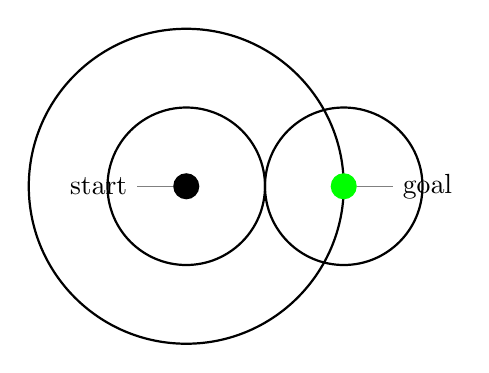
\begin{tikzpicture}
    \draw[black,thick] (0,0) circle (1cm);
    \draw[black,thick] (0,0) circle (2cm);
    \draw[black,thick] (2,0) circle (1cm);

    % \node[fill=black] (start) at (0,0) circle (1mm);
    \node[shape=circle,fill=black,pin={left:start}] (start) at (0,0) {};
    \node[shape=circle,fill=green,pin={right:goal}] (goal) at (2,0) {};
  \end{tikzpicture}
  \begin{itemize}
  \item<1> BFS?
  \item<1> DFS? 
  \end{itemize}
\end{center}
\end{frame}

\begin{frame}{Bidirectional Search}
  \begin{itemize}
   
  \item Alternate between goal and start nodes
  \item Instead of using goal\_test() we check if the current node is
    on the fringe of one search tree
  \end{itemize}
  Code
\end{frame}
\section{Heuristics}
\begin{frame}{Heuristics}
  \begin{itemize}
  \item Can we make smarter 
    decisions about which nodes to
    expand?
  \item That depends on the problem
  \item What makes one node more promising than another?
   \begin{itemize}
   \item<2-> Maze: how far from the end are we?
   \item<3-> Computer Algebra System: how similar is the expression to
     what we want?
   \item<4-> Chess: Which board position gives us the biggest point
     difference in our favor?  (more on this later)
   \end{itemize}
  \end{itemize}
\end{frame}
\begin{frame}{A*}
  % \scriptsize \verbatiminput{a-star.py}
  \normalsize
\end{frame}
\begin{frame}
  \frametitle{A*}
  \begin{alertblock} {Warning!}
    If you are looking for the \textbf{optimal} solution, the heuristic must
    have special properties
  \end{alertblock}
    In order to get a \emph{shortest} path the heuristic must \textbf{never}
  underestimate the actual distance, $h^*(x)$
  \begin{align*}
    \forall x :h^*(x) \le  h(x)
  \end{align*}
\end{frame}

\begin{frame}
  \frametitle{A*}

  \begin{figure}
    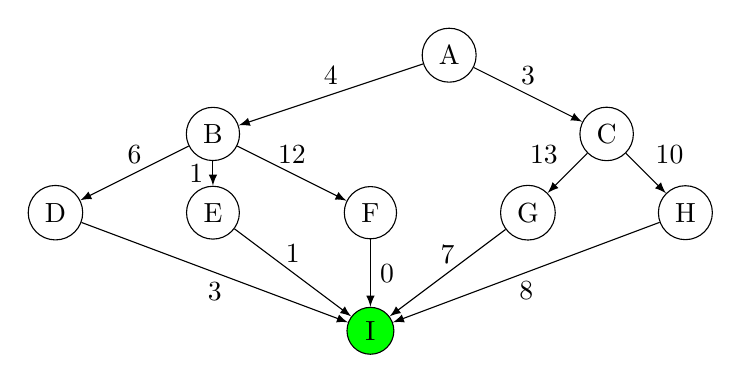
\begin{tikzpicture}
      \tikzset{>=latex}
      
      \node[shape=circle,draw=black](A) at (0,0) {A};
      \node[shape=circle,draw=black](B) at (-3, -1) {B};
      \node[shape=circle,draw=black](C) at (2, -1) {C};
      \node[shape=circle,draw=black](D) at (-5,-2) {D};
      \node[shape=circle,draw=black](E) at (-3, -2) {E};
      \node[shape=circle,draw=black](F) at (-1, -2) {F};
      \node[shape=circle,draw=black](G) at (1,-2) {G};
      \node[shape=circle,draw=black](H) at (3, -2) {H};
      \node[shape=circle,draw=black,fill=green] (I) at (-1, -3.5) {I};

      \draw [->] (A) edge node[above]{3} (C);
      \draw [->] (A) edge node[above]{4} (B);
      \draw [->] (B) edge node[above]{6} (D);
      \draw [->] (B) edge node[left]{1} (E);
      \draw [->] (B) edge node[above]{12} (F);
      \draw [->] (C) edge node[above left]{13} (G);
      \draw [->] (C) edge node[above right]{10} (H);
      \draw [->] (D) edge node[below]{3} (I);
      \draw [->] (E) edge node[above]{1} (I);
      \draw [->] (F) edge node[right]{0} (I);
      \draw [->] (G) edge node[above]{7} (I);
      \draw [->] (H) edge node[below]{8} (I);
    \end{tikzpicture}
  \end{figure}
  Search Order: A $\rightarrow$ B $\rightarrow$ F $\rightarrow$ I
\end{frame}
\begin{frame}{Beam Search}
  \begin{itemize}
  \item A* is an extension of breadth first search
  \item Can we improve it by eliminating the limitations that come
    with BFS?
  \end{itemize}
\end{frame}
\begin{frame}{Example Time!}
\end{frame}
\section{Adversarial Search} 
\begin{frame}{Adversarial Search}
  \begin{itemize}
  \item A.K.A Minimax
  \item Used to play games
  \item We are not the only one who can choose the next action!
  \end{itemize}
\end{frame}
\begin{frame}
  \frametitle{Adversarial Search} 
  2-player game:
  \begin{figure}
    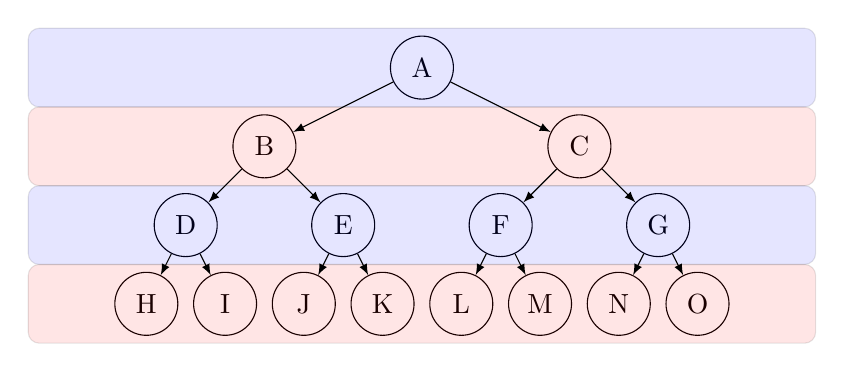
\begin{tikzpicture}[->,>=latex]
      \tikzstyle{node}=[shape=circle,draw=black,minimum size=8mm];
      \tikzstyle{rect}=[rounded corners,draw=black,opacity=0.1];
      
      
      \node[node](A) at (0,0) {A};
      \node[node](B) at (-2, -1) {B};
      \node[node](C) at (2, -1) {C};
      \node[node](D) at (-3,-2) {D};
      \node[node](E) at (-1, -2) {E};
      \node[node](F) at (1,-2) {F};
      \node[node](G) at (3, -2) {G};
      \node[node](H) at (-3.5, -3) {H};
      \node[node](I) at (-2.5, -3) {I};
      \node[node](J) at (-1.5, -3) {J};
      \node[node](K) at (-0.5, -3) {K};
      \node[node](L) at (0.5, -3) {L};
      \node[node](M) at (1.5, -3) {M};
      \node[node](N) at (2.5, -3) {N};
      \node[node](O) at (3.5, -3) {O};


      \path[rect,fill=blue] (-5,0.5) rectangle (5,-0.5);
      \path[rect,fill=red] (-5,-0.5) rectangle (5,-1.5);
      \path[rect,fill=blue] (-5,-1.5) rectangle (5,-2.5);
      \path[rect,fill=red] (-5,-2.5) rectangle (5,-3.5);

      \path (A) edge (C);
      \path (A) edge (B);
      \path (B) edge (D);
      \path (B) edge (E);
      \path (C) edge (F);
      \path (C) edge (G);
      \path (D) edge (H);
      \path (D) edge (I);
      \path (E) edge (J);
      \path (E) edge (K);
      \path (F) edge (L);
      \path (F) edge (M);
      \path (G) edge (N);
      \path (G) edge (O);

    \end{tikzpicture}
  \end{figure}
\end{frame}

\begin{frame}
  \frametitle{Adversarial Search}
  Minimax
  \begin{figure}
    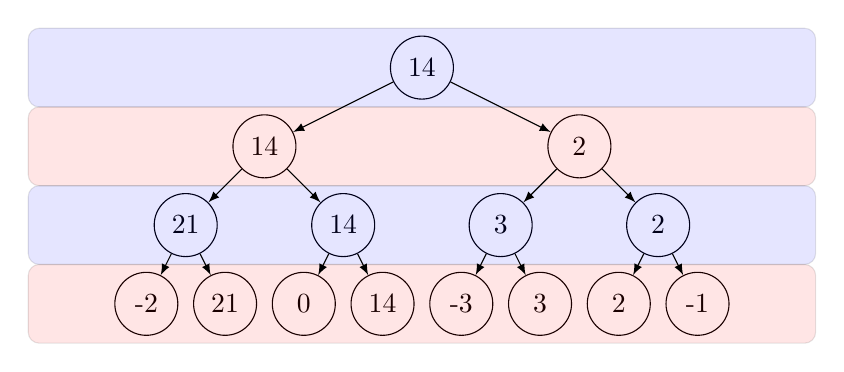
\begin{tikzpicture}[->,>=latex]
      \tikzstyle{node}=[shape=circle,draw=black,minimum size=8mm];
      \tikzstyle{rect}=[rounded corners,draw=black,opacity=0.1];
      
      
      \node[node](A) at (0,0) {14};
      \node[node](B) at (-2, -1) {14};
      \node[node](C) at (2, -1) {2};
      \node[node](D) at (-3,-2) {21};
      \node[node](E) at (-1, -2) {14};
      \node[node](F) at (1,-2) {3};
      \node[node](G) at (3, -2) {2};
      \node[node](H) at (-3.5, -3) {-2};
      \node[node](I) at (-2.5, -3) {21};
      \node[node](J) at (-1.5, -3) {0};
      \node[node](K) at (-0.5, -3) {14};
      \node[node](L) at (0.5, -3) {-3};
      \node[node](M) at (1.5, -3) {3};
      \node[node](N) at (2.5, -3) {2};
      \node[node](O) at (3.5, -3) {-1};


      \path[rect,fill=blue] (-5,0.5) rectangle (5,-0.5);
      \path[rect,fill=red] (-5,-0.5) rectangle (5,-1.5);
      \path[rect,fill=blue] (-5,-1.5) rectangle (5,-2.5);
      \path[rect,fill=red] (-5,-2.5) rectangle (5,-3.5);


      \path (A) edge (C);
      \path (A) edge (B);
      \path (B) edge (D);
      \path (B) edge (E);
      \path (C) edge (F);
      \path (C) edge (G);
      \path (D) edge (H);
      \path (D) edge (I);
      \path (E) edge (J);
      \path (E) edge (K);
      \path (F) edge (L);
      \path (F) edge (M);
      \path (G) edge (N);
      \path (G) edge (O);

    \end{tikzpicture}
  \end{figure}
\end{frame}

\begin{frame}{Example Time!}
  text-based Tic Tac Toe example
\end{frame}
\begin{frame}
  \frametitle{Chess}
  \begin{itemize}
  \item Add alpha-beta pruning to tic-tac-toe
  \item Transplant algorithm into graphical chess program
  \end{itemize}
\end{frame}
\begin{frame}{Alpha Beta Pruning}
  \begin{itemize}
  \item Are there nodes that can can be skipped?
  \item<2-> Yes! Sometimes...
  \end{itemize}
\end{frame}
\begin{frame}
  \frametitle{Example Time!}
\end{frame}
\end{document}
\begin{frame}
  \frametitle{Local Search}
  
\end{frame}
%%% Local Variables:
%%% mode: latex
%%% TeX-master: t
%%% End:
